\ifthenelse{\boolean{scanPernyataanOrisinalitas}}
{
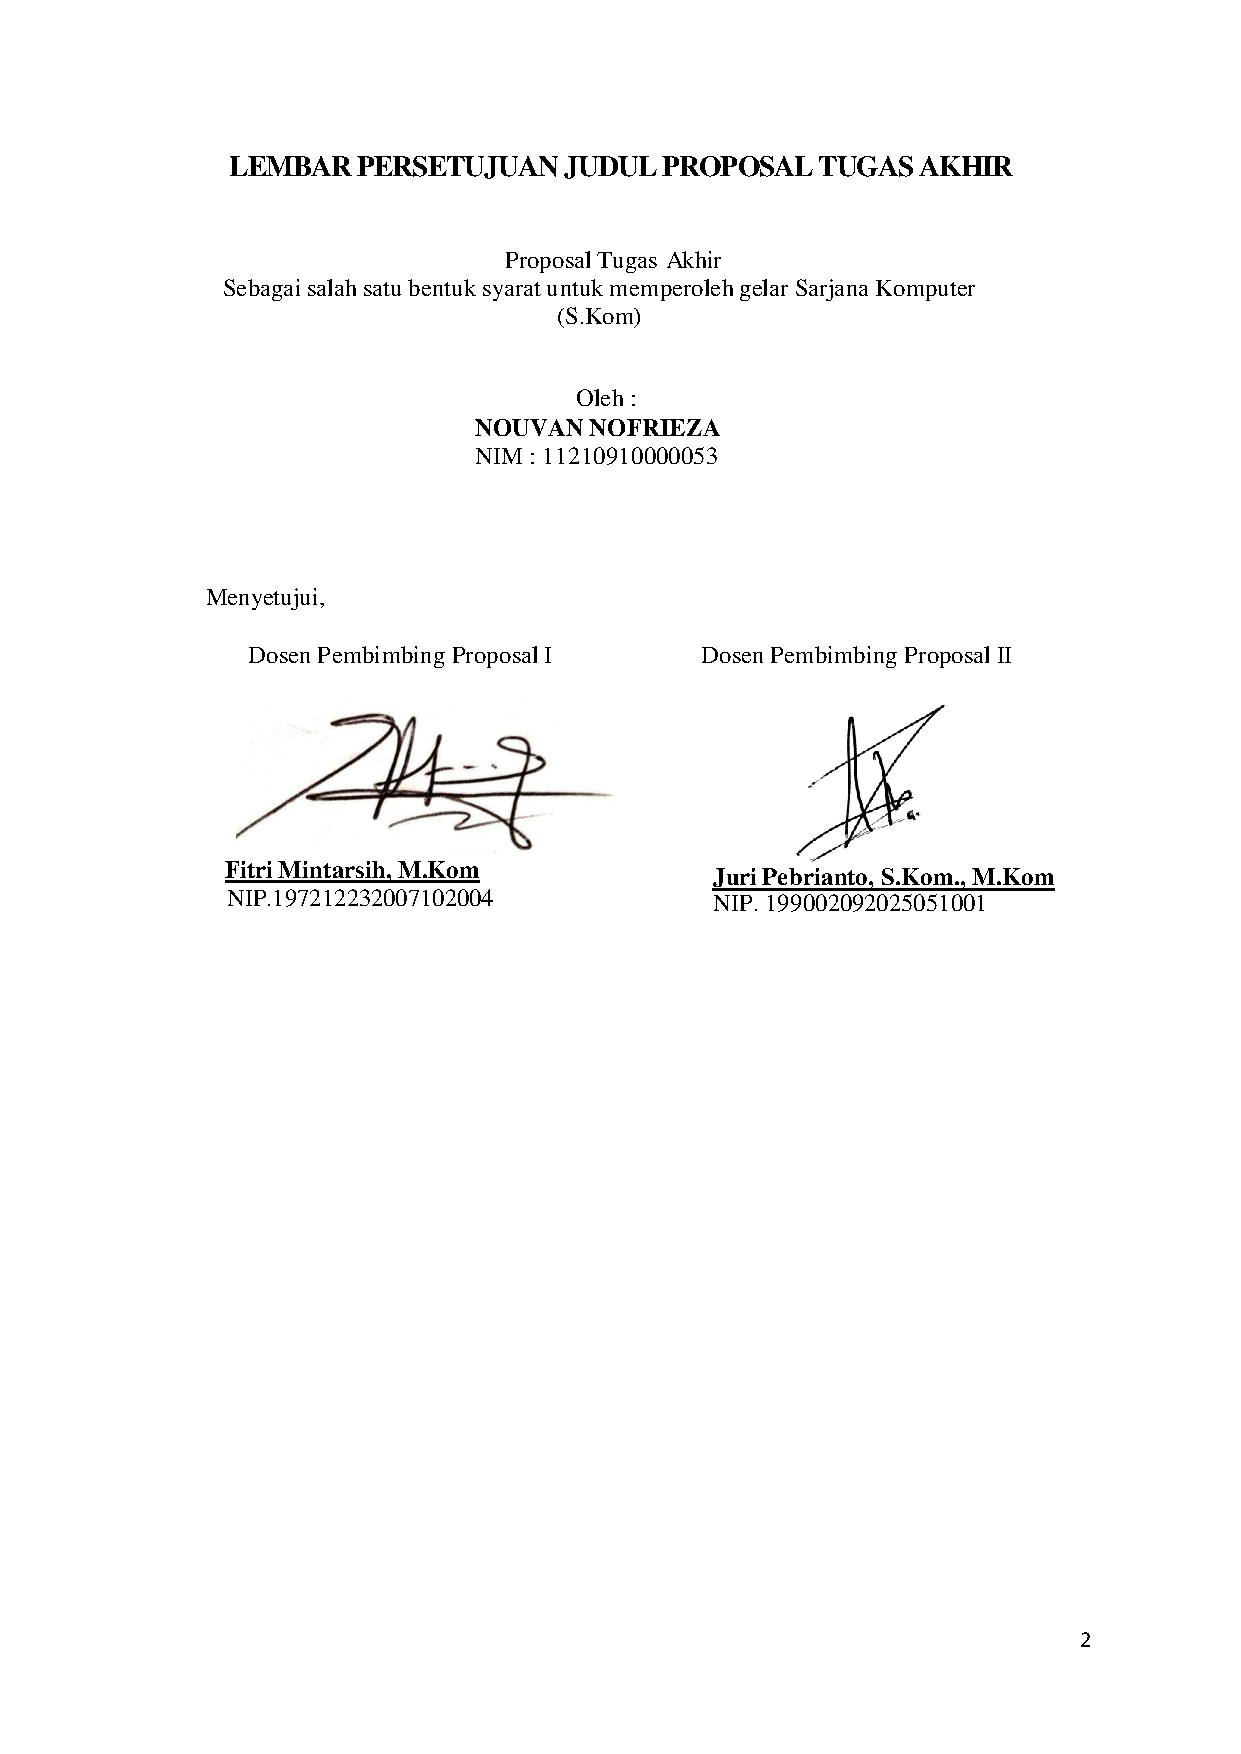
\includepdf[pages=1]{signature/pernyataan_orisinalitas.pdf}
}
{
% ===== TEMPLATE LATEX PERNYATAAN ORISINALITAS =====

\begin{center}
{\Large \textbf{LEMBAR PERNYATAAN ORISINALITAS}}
\end{center}

\vspace{1.5cm}
\noindent
Saya yang bertanda tangan di bawah ini:

\vspace{0.7cm}

\noindent
\begin{tabularx}{\textwidth}{>{\RaggedRight\arraybackslash}p{3.2cm} p{0.4cm} >{\RaggedRight\arraybackslash}X}
Nama & : & \namaPenulis \\
NIM & : & \nim \\
Program Studi & : & \programStudi \\
Fakultas & : & \fakultas \\
Judul Skripsi & : & \judulSkripsiID \\
\end{tabularx}

\vspace{1.5cm}
\noindent
Dengan ini menyatakan bahwa skripsi yang saya tulis ini benar-benar merupakan  hasil karya saya sendiri dan bukan merupakan plagiarisme dari karya orang lain, 
baik sebagian maupun seluruhnya. Apabila di kemudian hari terbukti bahwa skripsi ini merupakan hasil plagiarisme, 
maka saya bersedia menerima sanksi sesuai dengan ketentuan yang berlaku di 
Universitas Islam Negeri Syarif Hidayatullah Jakarta.

\vspace{2.5cm}

\begin{flushright}
\kota, \tanggalPernyataanOrisinalitas

\vspace{0.4cm}

{\color{materaigray}
\textit{Tempel Materai\\Rp10.000\\di area ini}
}

\vspace{0.4cm}

\rule{4cm}{0.4pt}\\
\namaPenulis
\end{flushright}

\newpage
}

\addcontentsline{toc}{chapter}{LEMBAR PERNYATAAN ORISINALITAS}